\documentclass[10pt,a4paper]{article}
\usepackage[utf8]{inputenc}
\usepackage[ngerman]{babel}
\usepackage[T1]{fontenc}
\usepackage{amsmath}
\usepackage{amsfonts}
\usepackage{amssymb}
\usepackage{graphicx}
\usepackage{lmodern}
\usepackage{physics}
\usepackage[left=1cm,right=1cm,top=1.5cm,bottom=1.2cm]{geometry}
\usepackage{siunitx}
\usepackage{fancyhdr}
\usepackage{enumerate}
\usepackage{mhchem}
\usepackage{mathtools}
\usepackage{graphicx}
\usepackage{float}
\usepackage[table]{xcolor}
\usepackage{mdframed}
\usepackage{csquotes}
\usepackage{trfsigns}
\usepackage{capt-of}
\usepackage{adjustbox}
\usepackage{verbatim}

\sisetup{locale=DE}
\sisetup{per-mode = symbol-or-fraction}
\sisetup{separate-uncertainty=true}
\DeclareSIUnit\year{a}
\DeclareSIUnit\clight{c}
\mdfdefinestyle{exercise}{
	backgroundcolor=black!10,roundcorner=8pt,hidealllines=true,nobreak
}

\begin{document}
\twocolumn
\pagestyle{fancy}
% \lhead{DSV Formelsammlung, Stand {\input{\string"| date + " %Y-%d-%m" \string"}}}
\lhead{Formelsammlung Mathe, \today}
\rhead{Sedlmeier, Toni}
\section{Wahrscheinlichkeiten}
%%%%%%%%%%%%%%%%%%%%%%%%%%%%%%%%%%%%% Elementare System-Eigenschaften %%%%%%%%%%%%%%%%%%%%%%%%%%%%%%%%%%%%%%%%%%%%
  \subsection{Axiome von Kolmogoroff}
  \begin{enumerate}[(K1)]
      \item $P(A) \geq 0$ \ \ Nichtnegativität
      \item $P(\Omega) = 1$ \ \ Normierung
      \item Falls $A \cap B = 0 \rightarrow P(A\cap B)=P(A)+P(B) $ \ \ Additivität
  \end{enumerate}
  
  \subsection{Rechenregeln}
  \begin{mdframed}[style=exercise]
    \begin{align}
        P(A \cup B ) = P(A) + P(B) - P(A \cap B )
    \end{align}
  \end{mdframed}
    $A_1$ ... $A_n$ paarweise disjunkt (keine Scnittfläche)
  \begin{mdframed}[style=exercise]
    \begin{align}
        P(A_1 \cup A_2 \cup ... A_n) = P(A_1) + P(A_2) + ... +P(A_n)
    \end{align}
  \end{mdframed}
  falls nicht disjunkt Schnittfläche abziehen
  \begin{mdframed}[style=exercise]
    \begin{align}
        P(A \cup B ) = P(A) + P(B) - P(A\cap B)
    \end{align}
  \end{mdframed}
  
  \begin{mdframed}[style=exercise]
    \begin{align}
        P(A \cup B ) = 1 - P(\overline{A} \cap \overline{B})
    \end{align}
  \end{mdframed}


  \subsection{Bedingte Wahrscheinlichkeiten}
  \begin{mdframed}[style=exercise]
    \begin{align}
    P (A \cap B) = P (B) \cdot P (A\ |\ B).
    \end{align}
  \end{mdframed}

  \subsubsection{Baumdiagramm}
  \begin{center}
      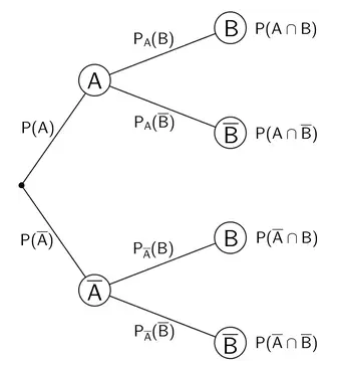
\includegraphics[width=.22\textwidth]{./img/baum.png}
  \end{center}
  \subsubsection{4-Felder Tafel}
  \begin{center}
      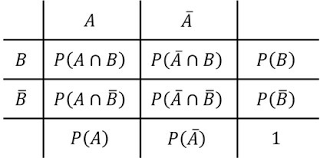
\includegraphics[width=.22\textwidth]{./img/vier.png}
  \end{center}

  \subsubsection{Stoch. Unabhängigkeit}
  \begin{mdframed}[style=exercise]
    \begin{align}
        P (A \cap B) = P(A) \cdot P(B)
    \end{align}
  \end{mdframed}

  \subsection{Satz von Bayes}
  \begin{mdframed}[style=exercise]
    \begin{align}
        P(A) = \displaystyle\sum_{i=1}^{n} P(A|B_i) \cdot P(B_i) \\
        P(B) = \displaystyle\sum_{i=1}^{n} P(B|A_i) \cdot P(A_i)
    \end{align}
  \end{mdframed}

  \begin{mdframed}[style=exercise]
    \begin{align}
        P (A_i \ |\ B) = \frac{P(A_i \cap B)}{P(B)} = \frac{P(B | A_i) \cdot P(A_i)}{P(B)}
    \end{align}
  \end{mdframed}

  \newpage

  \section{Diskrete Verteilungen}
  $E$ = Ereignis\\
  $\omega$ = Ergebnis\\
  $\Omega$ = Ergebnisraum\\

  Bsp: Würfeln
  \begin{center}
      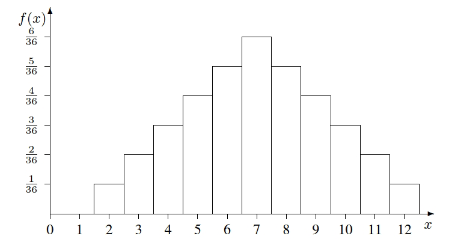
\includegraphics[width=.22\textwidth]{./img/wuerfel.png}
  \end{center}
Wahrscheinlichkeitsdichtefunktion $f_X(x)$ beschreibt die Wahrscheinlichkeit $P(X=x_i)$, 
dass die ZV $X$ den Wert $x_i$ annimmt
  \begin{mdframed}[style=exercise]
    \begin{align}
        f_X(x):=\left\{\begin{array}{ll} P(X=x_i) = p_i,  & x = x_i\in W(X) \\ \\
         0, & sonst\end{array}\right. .
    \end{align}
  \end{mdframed}

\subsection{Maßzahlen diskreter Verteilungen}
\subsubsection{Erwartungswert}
  \begin{mdframed}[style=exercise]
    \begin{align}
        E(aX +b) &= aE(X)+b \\
        E(X \cdot Y) &= E(X) \cdot E(Y)\\
        E(X + Y) &= E(X) + E(Y)
    \end{align}
  \end{mdframed}

\subsubsection{Varianz}
  \begin{mdframed}[style=exercise]
    \begin{align}
        Var(aX) &= a^2 Var(X) \\
        Var(X + a) &= Var(X)  \\
        Var(X + Y) &=  Var(X) + Var(Y)\\
    \end{align}
  \end{mdframed}

  \begin{mdframed}[style=exercise]
    \begin{align}
        \mu_X &= E[X] = \sum_{i \geq 1} x_i f_X(x_i) = \sum_{i \geq 1} x_i p_i
    \end{align}
  \end{mdframed}

  \begin{mdframed}[style=exercise]
    \begin{align}
        \sigma_X^2 &= E[(x-\mu_x)^2] = E[x^2]-\mu_x^2 \\ 
        \sigma_X^2 &= \sum_{i \geq 1} (x_i -E(X))^2 f_X(x_i) \\
        \sigma_X^2 &= \sum_{i \geq 1} (x_i -E(X))^2 p_i
    \end{align}
  \end{mdframed}

  \begin{mdframed}[style=exercise]
    \begin{align}
        E[X^2] &= \sum_{i \geq 1} x_i^2 p_i\\
    \end{align}
  \end{mdframed}

\subsubsection{Modus}
Lokales Maximum der Verteilung $f_X(x)$ ist Modus $X_{mod}$ \\
Bsp: 2-Mal Würfeln $X_{mod} = 7$

\subsection{Diskrete Gleichverteilung}
Alle Werte mit gleicher Wahrscheinlichkeit \\
\textbf{Wertebereich:} $W(X)= \{x_1 ... x_n \}$
  \begin{mdframed}[style=exercise]
    \begin{align}
        f_X(x):=\left\{\begin{array}{ll} \frac{1}{n},  & x \in W(X) \\ \\
         0, & sonst\end{array}\right. .
    \end{align}
  \end{mdframed}

  \begin{mdframed}[style=exercise]
    \begin{align}
        E(X) &= \frac{1}{n} \sum_{i=1}^n x_i \\
        Var(X) &= \frac{1}{n} \sum_{i=1}^n x_i^2 
    \end{align}
  \end{mdframed}

\subsection{Bernoulli - Verteilung}
Zufallsprozess mit 2 möglichen Ausgängen (z.B Prüfungen) \\
\textbf{Wertebereich:} $W(X)= \{0;1 \}$\\
\textbf{Notation:} X $\sim$ Ber(p) mit p = P(A) 
  \begin{mdframed}[style=exercise]
    \begin{align}
        f_X(x):=\left\{\begin{array}{ll} P(X=0) = p_A \\ \\
         P(X=1) = 1-p_A \end{array}\right. .
    \end{align}
  \end{mdframed}

  \begin{mdframed}[style=exercise]
    \begin{align}
        E(X) &= p \\
        Var(X) &= p(1-p) 
    \end{align}
  \end{mdframed}

\subsection{Binomial - Verteilung}
Zählen der Ereigniseintritte bei $n$ unabhängigen Bernoullivorgängen \\
\textbf{Wertebereich:} $W(X)= \{0 ... n \}$\\
\textbf{Notation:} X $\sim$ Bin(n,p) \\
\textbf{Parameter:} \begin{itemize}
    \item $p$ = WSK des Bernoullivorgangs 
    \item $n$ = Anzahl Wiederholungen 
    \item $x$ = Anzahl Ereigniseintritte 
\end{itemize}
  \begin{mdframed}[style=exercise]
    \begin{align}
        f_X(x):=\left\{\begin{array}{ll} \binom{n}{x} \cdot p^x \cdot (1-p)^{n-x}, & n \in W(X) \\ \\
        0, & sonst \end{array}\right. .
    \end{align}
  \end{mdframed}

  \begin{mdframed}[style=exercise]
    \begin{align}
        E(X) &= n\cdot p \\
        Var(X) &= n\cdot p (1-p) 
    \end{align}
  \end{mdframed}
  Additionseigenschaft:
  \begin{mdframed}[style=exercise]
    \begin{align}
        X   &\sim Ber(n,p)\\
        Y   &\sim Ber(m,p)\\
        X+Y &\sim Ber(n+m,p)
    \end{align}
  \end{mdframed}

\subsection{Poisson - Verteilung}
Anzahl an Ereigniseintritten in fixen Zeitintervallen \\
\textbf{Wertebereich:} $W(X)= \mathbb{N}$ \\
\textbf{Notation:} $X \sim Poi(\lambda)$ \\
\textbf{Parameter:} \begin{itemize}
    \item $\lambda$ = Rate
\end{itemize}

  \begin{mdframed}[style=exercise]
    \begin{align}
        f_X(x):=\left\{\begin{array}{ll} \frac{\lambda^x}{x!} e^{-\lambda}, & n \in W(X) \\ \\
        0, & sonst \end{array}\right. .
    \end{align}
  \end{mdframed}

  \begin{mdframed}[style=exercise]
    \begin{align}
        E(X) &= \lambda \\
        Var(X) &= \lambda 
    \end{align}
  \end{mdframed}
\textbf{Eigenschaften:}
\begin{enumerate}
    \item Additionseigenschaft
  \begin{mdframed}[style=exercise]
    \begin{align}
        X   &\sim Poi(\lambda)\\
        Y   &\sim Poi(\mu)\\
        X+Y &\sim Poi(\lambda+\mu)
    \end{align}
  \end{mdframed}
  \item Anzahl Ereignisse innerh. $t\sim Poi(\lambda) \rightarrow Poi(t\lambda)$ 
\end{enumerate}

  \newpage

\subsection{Geometrische - Verteilung}
Anzahl an Wiederholungen bis zum 1. Ereigniseintritt von A
\textbf{Wertebereich:} $W(X)= \mathbb{N}$ \\
\textbf{Notation:} $X \sim Geo(p)$ \\
\textbf{Parameter:} \begin{itemize}
    \item $ p=P(A)$ = WSK
\end{itemize}

  \begin{mdframed}[style=exercise]
    \begin{align}
        f_X(x):=\left\{\begin{array}{ll} (1-p)^{x-1} \cdot p, & n \in W(X) \\ \\
        0, & sonst \end{array}\right. .
    \end{align}
  \end{mdframed}

  \begin{mdframed}[style=exercise]
    \begin{align}
        E(X) &= \frac{1}{p} \\
        Var(X) &= \frac{1-p}{p^2}
    \end{align}
  \end{mdframed}
\textbf{hilfreich:}\\
Ereignis tritt spätestens mit der x-ten Wiederholung
  \begin{mdframed}[style=exercise]
    \begin{align}
        P(X \leq x) = 1-(1-p)^x
    \end{align}
  \end{mdframed}

  \newpage
  \section{Stetige Zufallsvariablen}

    \subsection{Maßzahlen stetiger Zufallsvariablen}
    \subsubsection{Wahrscheinlichkeitsdichtefunktion}
    Wahrscheinlickkeit $P(x_u \leq x \leq x_o )$, dass $x \in [x_u,x_o]$ 
      \begin{mdframed}[style=exercise]
        \begin{align}
            P(a \leq X \leq b ) &= \displaystyle\int_{a}^{b} f_X(x) dx \\
            1 &= \displaystyle\int_{-\infty}^{\infty} f_X(x)dx 
        \end{align}
      \end{mdframed}

    \subsubsection{Wahrscheinlichkeitsverteilungsfunktion}
    Wahrscheinlickkeit $P(x_u \leq x \leq x_o )$, dass $x \in [x_u,x_o]$ 
      \begin{mdframed}[style=exercise]
        \begin{align}
            F_X(x) &= \displaystyle\int_{-\infty}^{x} f_X(u)du
        \end{align}
      \end{mdframed}

    \subsubsection{Erwartungswert $\mu_x$, Varianz $\sigma_x^2$}
    Formeln gelten nur für \textbf{stationäre} Zufallsvariablen bzw stochastische Prozesse
      \begin{mdframed}[style=exercise]
        \begin{align}
            \mu_X &= E[X] = \displaystyle\int_{-\infty}^{\infty} x f_X(x) dx \\
             E[X^2] &= \displaystyle\int_{-\infty}^{\infty} x^2 f_X(x) dx \\
            \sigma_X^2 &= E[(x-\mu_X)^2] = E[X^2]-\mu_X^2 \\
            \sigma_X^2 &= \displaystyle\int_{-\infty}^{\infty} (x-\mu_x)^2 \ f_x(\alpha) d\alpha
        \end{align}
      \end{mdframed}

      \subsubsection{Transformation einer ZV}
      Eine ZV $X$ wird mit einer Funktion $g$ auf neue ZV $Y$ abgebildet (transformiert)
      \begin{mdframed}[style=exercise]
        \begin{align}
            E(Y) &= E(g(X)) =\displaystyle\int_{-\infty}^{\infty} g(x) \cdot f_X(x) dx \\
        \end{align}
      \end{mdframed}
      Falls $g(x) = ax+b$
      \begin{mdframed}[style=exercise]
        \begin{align}
            E(Y) &= E(aX+b) = a \cdot E(X) + b \\
        \end{align}
      \end{mdframed}

      \subsubsection{Quantile und Median}
      \textbf{Quantil:} Wert $x_p$, der mit W $p$ unterschritten und W $(1-p)$ überschritten wird. \\
      \textbf{Median:} Für $p=0.5$ erhält man den Median.
      \begin{center}
          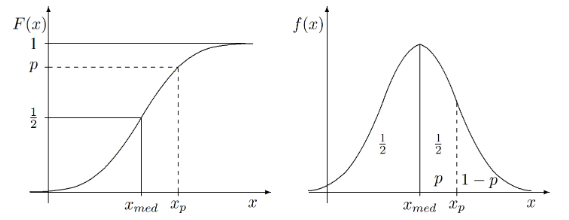
\includegraphics[width=.5\textwidth]{./img/quant.png}
      \end{center}

  \subsubsection{Zentrierung und Standartisierung}
  Eine ZV $X$ ist zentriert, wenn $E(X) = 0$.
  X ist standartisiert, wenn $E(X) = 0$ und $Var(X) = 1$
  Standartisierung von $X$ führt zu $Z$ (zentriert):
      \begin{mdframed}[style=exercise]
        \begin{align}
            Z = \frac{X-E(X)}{\sqrt{Var(X)}}
        \end{align}
      \end{mdframed}

\subsection{Kontinuierliche Gleichverteilung}
Alle Werte aus einem Intervall gleich wahrscheinlich \\
\textbf{Notation:} $X \sim U(a,b)$ \\
\textbf{Parameter:} \begin{itemize}
    \item $a$ = untere Grenze
    \item $b$ = obere Grenze
\end{itemize}

  \begin{mdframed}[style=exercise]
    \begin{align}
        f_X(x):=\left\{\begin{array}{ll} \frac{1}{b-a}, & x \in \{a;b\} \\ \\
        0, & sonst \end{array}\right. .
    \end{align}
  \end{mdframed}
  
  \begin{mdframed}[style=exercise]
    \begin{align}
        F_X(x):=\left\{
            \begin{array}{ll} 
                0, & x < a \\ \\
                \frac{x-a}{b-a}, & x \in \{a;b\} \\ \\
                1, & x > b 
            \end{array}
            \right. .
    \end{align}
  \end{mdframed}

  \begin{mdframed}[style=exercise]
    \begin{align}
        E(X) &= \frac{a+b}{2} \\
        Var(X) &= \frac{b-a}{12}
    \end{align}
  \end{mdframed}


  \newpage

\subsection{Normalverteilung (Gaußverteilung)}
\textbf{Notation:} $X \sim N(\sigma,\mu)$ \\
\textbf{Parameter:} \begin{itemize}
    \item $\sigma$ = Varianz
    \item $\mu$ = Erwartungswert
\end{itemize}
  \begin{mdframed}[style=exercise]
    \begin{align}
        f_x(\alpha) = \frac{1}{\sigma_x \cdot \sqrt{2\pi}} \cdot e^{-\frac{1}{2} \cdot \left( \frac{\alpha - \mu_x}{\sigma_x}\right)^2}
    \end{align}
  \end{mdframed}
      \begin{center}
          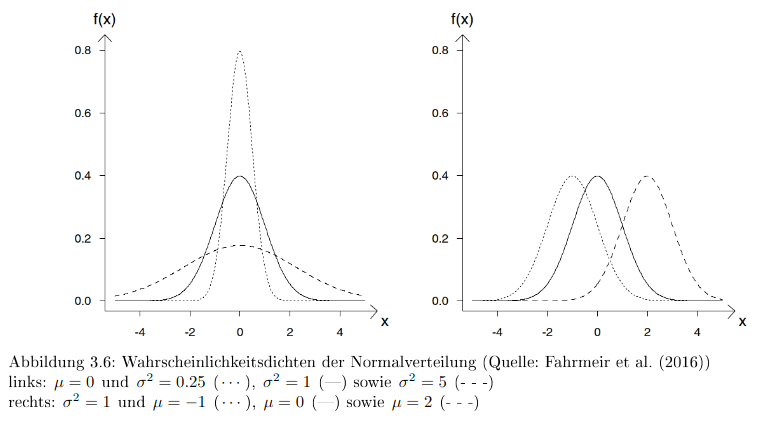
\includegraphics[width=.5\textwidth]{./img/norm.png}
      \end{center}
Normalverteilung symmetrisch um Erwartungswert $\mu$
  \begin{mdframed}[style=exercise]
    \begin{align}
        f(\mu - x) = f (\mu + x) \ \ \ \ \forall x \in \mathbb{R}
    \end{align}
  \end{mdframed}
Verteilungsfuntion $F(x)$ kann nicht analytisch bestimmt werden
außer $\mu = 0$ und $\sigma = 1\rightarrow$ \textbf{Standartnormalverteilung} 
$\rightarrow$ Tabelle!


\subsubsection{$k\sigma$-Intervalle}
Prozentualer Anteil der Wahrscheinlickkeitsmasse
  \begin{mdframed}[style=exercise]
    \begin{align}
        [\mu -k\sigma , \mu + k\sigma]
    \end{align}
  \end{mdframed}
    \begin{center}
        \begin{tabular}{ |c|c| } 
         \hline
            $1\sigma$ & 66,27\% \\ 
         \hline
            $2\sigma$ & 95,45\% \\ 
         \hline
            $3\sigma$ & 99,73\% \\ 
         \hline
        \end{tabular}
    \end{center}

\subsubsection{Berechnung von W mit $\Phi$}
Eine normalverteilte ZV $X\sim N(\mu_X,\sigma^2_X)$ soll in den Grenzen $a$ 
und $b$ ausgewertet werden. ges: $P(a\leq X \leq b)$ \\
$X$ kann zu $U\sim N(0,1)$ zentriert werden:
  \begin{mdframed}[style=exercise]
    \begin{align}
        a^* = \frac{a-\mu}{\sigma}\\
        b^* = \frac{b-\mu}{\sigma}
    \end{align}
  \end{mdframed}

  \begin{mdframed}[style=exercise]
    \begin{align}
        P(a\leq X \leq b) = P(a^*\leq U \leq b^*) =
        \Phi(a^*) - \Phi(b^*)
    \end{align}
  \end{mdframed}

\subsubsection{Quantile der Standartnormalverteilung}
Finde p-Quantil (obere Schranke) $x_p$ einer ZV $X$ zu gegebener W $p$ sodass gilt
  \begin{mdframed}[style=exercise]
    \begin{align}
        P(X\leq x_p) &= \Phi(x_p) = p \\
        x_p &= \ ?
    \end{align}
  \end{mdframed}
  $\rightarrow x_p$ Tabelle! \\
  Es gilt
  \begin{mdframed}[style=exercise]
    \begin{align}
        x_{1-p} = -x_p\\
        x_{p} = -x_{1-p}
    \end{align}
  \end{mdframed}

\subsection{Exponentialverteilung}
Dauer bis zum Ereigniseintritt
\textbf{Notation:} $X \sim Exp(\lambda)$ \\
\textbf{Parameter:} \begin{itemize}
    \item $\lambda$ = Rate
\end{itemize}
  \begin{mdframed}[style=exercise]
    \begin{align}
        f_X(x):=\left\{\begin{array}{ll} e^{-\lambda x}, & x \geq 0 \\ \\
        0, & x < 0 \end{array}\right. .
    \end{align}
  \end{mdframed}

  \begin{center}
      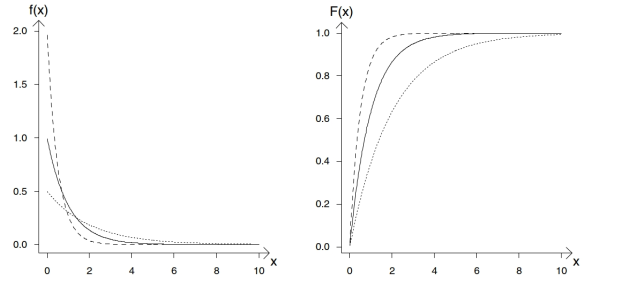
\includegraphics[width=.5\textwidth]{./img/expo.png}
  \end{center}

  \begin{itemize}
      \item gedächtnislos (egal wie lange man schon wartet)
      \item Alter/Verschleiß nicht berücksichtigt
      \item Median $x_{med} = 0.5$
  \end{itemize}

\subsection{Weibull-Verteilung}
Zeitabhängige Ausfallrate (Hazzard rate)
\textbf{Notation:} $X \sim Wei(\lambda, \alpha)$ \\
\textbf{Parameter:} \begin{itemize}
    \item $\lambda$ = Rate
    \item $\alpha$ = Erwartungswert
\end{itemize}
  \begin{mdframed}[style=exercise]
    \begin{align}
        f_X(x):=\left\{\begin{array}{ll} \lambda \alpha x^{\alpha -1}e^{-\lambda x^{\alpha}}, & x \geq 0 \\ \\
        0, & x < 0 \end{array}\right. .
    \end{align}
  \end{mdframed}

  \begin{mdframed}[style=exercise]
    \begin{align}
        F_X(x):=\left\{\begin{array}{ll} 1-e^{-\lambda x^{\alpha}}, & x \geq 0 \\ \\
        0, & x < 0 \end{array}\right. .
    \end{align}
  \end{mdframed}
  \begin{itemize}
      \item Lebensdauer, Ausfallrate
      \item Gedächtinisbehafte
  \end{itemize}

  \begin{center}
      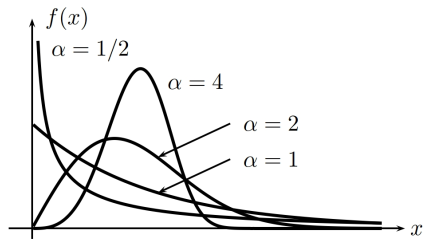
\includegraphics[width=.5\textwidth]{./img/weibull.png}
  \end{center}

  Ausfallrate (Hazzard rate) $a(t)$
  \begin{mdframed}[style=exercise]
    \begin{align}
        a(t) = \frac{f(t)}{1-F(t)} = \lambda \alpha t^{\alpha -1}
    \end{align}
  \end{mdframed}
  \begin{itemize}
      \item $\alpha >1$ Ausfallrate wächst (Alterung)
      \item $\alpha >1$ Ausfallrate fällt (Verjüngung)
  \end{itemize}


\end{document}
